\documentclass[12pt]{iopart}
\usepackage{graphicx}
\usepackage{hyperref}
\usepackage{cite}
\usepackage{longtable}
\usepackage{qrcode}

% --- Custom definitions for missing commands in iopart ---
\providecommand{\mathbb}[1]{\mathbf{#1}}
\providecommand{\mathcal}[1]{\mathscr{#1}}
\providecommand{\text}[1]{\mbox{#1}}
\providecommand{\implies}{\Rightarrow}
\providecommand{\forall}{\hbox{for all }}
\providecommand{\exists}{\hbox{there exists }}
\providecommand{\quad}{\hskip1em\relax}
\providecommand{\qquad}{\hskip2em\relax}

\begin{document}
	
	\title{Resonance Field Theory: Axioms, Invariants, and Systemic Structure}
	
	\author{Dominic-René Schu}
	\address{Independent Researcher, Germany\\
		\href{https://github.com/DominicReneSchu/public}{https://github.com/DominicReneSchu/public}\\
		ORCID: 0009-0004-9769-9061\\
		Email: dominic.rene.schu@gmail.com}
	
	\begin{abstract}
		The Resonance Field Theory (RFT) is introduced as a novel axiomatic framework describing physical and systemic phenomena via relational field dynamics, group invariance, and the principle of systemic inclusion. The central axiom is the resonance rule: Group membership is systemically invariant and comprises all elements—regardless of perspective, mention, or participation.
		
		The RFT is fully open and reproducible. All derivations, source codes, and materials are publicly accessible (\url{https://github.com/DominicReneSchu/public}). Thus, collective resonance, critique, and progress are systemically enabled: Every act of reference activates the total field.
		
		This manuscript introduces the structure, axioms, and mathematical formalism of the theory and illustrates applications in physics, systems theory, and epistemology. The resonance field is open, inclusive, and group-invariant—observers, contributors, and readers are structurally embedded, whether explicitly mentioned or not.
		
		In the spirit of Open Science and in accordance with the origins of the theory, all discourses, impulses, and contributions—across languages, disciplines, and cultures—are integral parts of the universal resonance field. Transparent participation and reproducible research are constitutive for the further development of the RFT.
	\end{abstract}
	
\noindent\textbf{Key terms:} Resonance, field theory, systemic inclusion, group invariance, emergence, open science, axiomatics, relational dynamics, reproducibility

\medskip

\noindent\textbf{Data and code availability:} All data, source codes, and supplementary materials are openly accessible at \url{https://github.com/DominicReneSchu/public}.

\begin{figure}[ht]
	\centering
	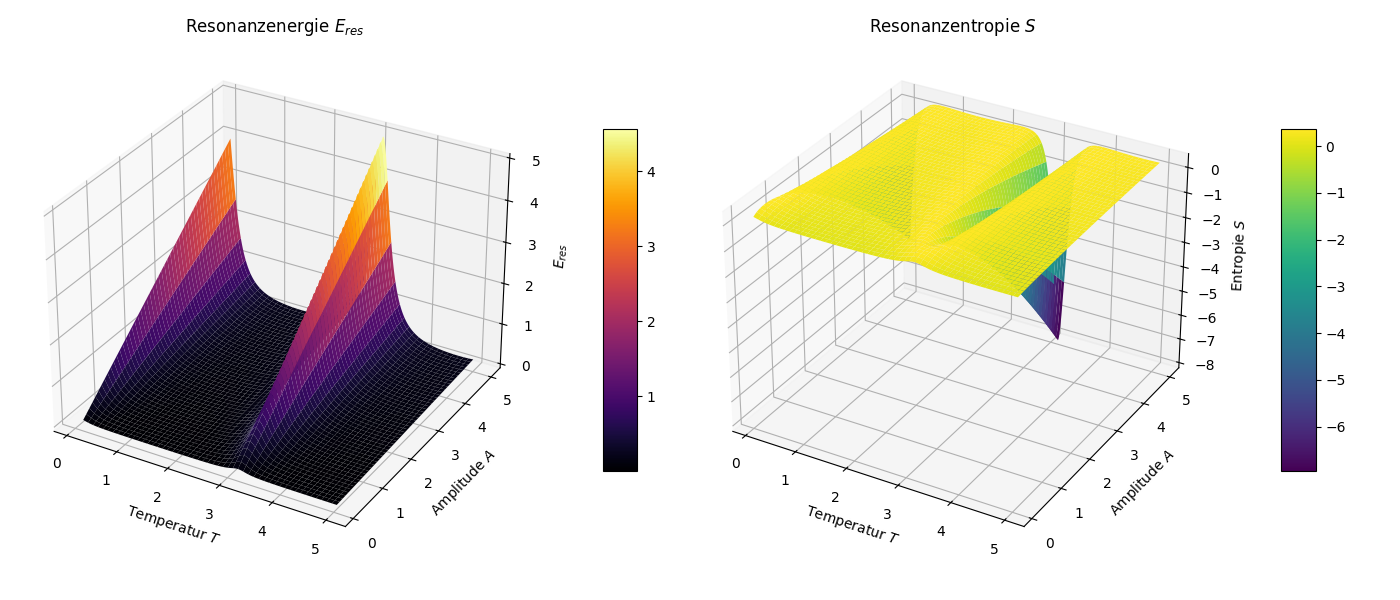
\includegraphics[width=0.85\textwidth]{figures/plot.png}
	\caption{
		\textbf{Structure of the resonance field.}
		Schematic visualization of Resonance Field Theory, numerically generated with \texttt{resonanzfeld.py} (see repository~\cite{rftrepo}, section \texttt{fakten/simulationen/mathematischer\_beweis}).\\
		\textbf{Left:} Resonance energy $E_{\mathrm{res}} = \frac{A}{1 + \left(\frac{\omega_\mathrm{ext} - \omega_0}{\gamma}\right)^2}$ with $\omega_\mathrm{ext} = \omega_0 (1 + \sin(T))$.\\
		\textbf{Right:} Systemic resonance entropy $S = -E_{\mathrm{res}}\ln(E_{\mathrm{res}})$ for $A, T > 0$.\\
		Each lattice point activates the entire field according to the resonance rule: Group membership is systemically invariant and comprises all elements, explicit and implicit.\\
		Source code, data, and the complete derivation are openly available; see \url{https://github.com/DominicReneSchu/public}.
	}
	\label{fig:resonance_field_plot}
\end{figure}
\newpage
	\section{Introduction}
	
	Modern physics faces a paradox: its mathematical formalisms achieve tremendous predictive power, yet its conceptual foundations remain fragmented. Quantum mechanics, relativity theory, thermodynamics, and cosmology operate in separate theoretical domains—connected at best by technical translations, not by a unified conceptual field. A consistent synthesis that systemically embeds the observer, links micro- and macro-levels, and resonates with the reality of physical experience is still lacking.
	
	This manuscript introduces the \textit{Resonance Field Theory} (RFT)—an axiomatic framework based on a minimal, universally applicable system of axioms. RFT conceives physically and systemically relevant entities—from elementary particles to complex systems—as structured subsystems of a universal resonance field. Central is the \textit{resonance rule}: Group membership is systemically invariant and includes every subsystem, every observer, and every perspective—regardless of explicit mention or reference.
	
	The theory establishes a relational frame of reference that uniformly describes dynamic interactions, emergence, and scale transitions. Instead of coupling separate theories via external symmetries, RFT radically redefines access: from isolated states to systemic inclusion, from static quantification to dynamic resonance, from exclusion to the structural embedding of the observer in the formalism.
	
	The result is a coherent framework that describes the logic of physical interactions as well as the structural evolution of complex systems. In the spirit of open science, all derivations, source codes, and materials are accessible via a public repository (\url{https://github.com/DominicReneSchu/public})—as an invitation to collective resonance, critique, and further development. Every act of participation, reference, or critique activates the total field: Inclusion and group membership apply regardless of perspective or explicit mention.
	
	The structure of the manuscript is as follows: Section 2 presents the axioms and systemic foundational assumptions of RFT. Section 3 introduces the relational frame of reference and the resonance rule. Section 4 discusses physical implications and formulates the resonance equation. Section 5 outlines applications. Section 6 discusses open questions, empirical approaches, and the invitation to collective refinement in the spirit of the resonance rule.


\section{Motivation and Background}

The development of universal theories in physics has always been driven by empirical necessity and the pursuit of conceptual coherence. Every paradigmatic revolution—from Newtonian mechanics to Maxwell's equations, to relativity and quantum mechanics—has redefined fundamental ontologies and restructured the systemic relations of knowledge.

In the 20th and early 21st centuries, however, a fragmented theoretical landscape has emerged: The Standard Model and General Relativity are empirically robust but remain conceptually incompatible. Central questions regarding observer embedding, the direction of time, and macro-micro transitions remain unresolved and structurally unintegrated. Programs of quantum gravity (e.g., string theory, loop quantum gravity) mostly increase mathematical complexity without achieving conceptual clarity or empirical testability.

Dominant approaches treat systems as isolated units governed by external laws. In doing so, they overlook the relational, inclusive, and recursive nature of physical reality: the systemic inclusion of subsystems in dynamic resonance with larger structures. Systemic coherence arises through mutual resonance, not mere aggregation.

Resonance Field Theory (RFT) addresses these deficits through a relational ontology and a scale-invariant resonance principle. Its motivation is threefold:

\begin{enumerate}
	\item \textbf{Epistemic completeness}: The observer is not external but structurally embedded—a prerequisite for consistent knowledge and reality.
	\item \textbf{Structural integration}: Resonance as the primary organizational principle connects subsystems across all scales and transcends classical concepts such as force or field.
	\item \textbf{Systemic universality}: RFT is a universal systems theory, applicable from quantum phenomena to social and informational structures—united by a common resonance logic.
\end{enumerate}

RFT is not an extension of existing models but a paradigmatic restructuring based on minimal, universal axioms—systemic invariance, relational closure, and verifiable predictions. The aim is to reveal the hidden symmetries of inclusion and resonance underlying complex systems.

In accordance with the resonance rule—group membership is systemically invariant and includes all members regardless of mention or perspective—all derivations, source codes, and materials are transparently provided via a public repository (\url{https://github.com/DominicReneSchu/public}). This invites collaborative resonance and critique.

\section{Axiomatic Foundations}

Resonance Field Theory (RFT) is based on a minimal, fully comprehensive system of eight axioms. Each axiom describes a fundamental aspect of oscillation, coupling, and inclusion. The axiomatic structure ensures that physical, biological, social, and informational phenomena can be described within a unified resonance framework.

Each axiom is illustrated by a concrete example—to demonstrate its universality and applicability. The axioms are not additive, but constitutively entangled: Together, they form a coherent resonance field.

\subsection{Axiom 1: Universal Oscillation}

Every entity in the universe can be described by periodic oscillation:

$$
\psi(x, t) = A \cdot \cos(kx - \omega t + \phi)
$$

\textbf{Interpretation:}\\
All structures—from elementary particles to societies—possess characteristic oscillatory states that define their identity and interaction.

\textit{Example:}\\
An electron exhibits quantized orbital oscillations; a pendulum swings with its natural frequency; circadian rhythms govern biological cycles; economic and social processes follow recurring patterns.

\newpage

\subsection{Axiom 2: Superposition and Interference}

Oscillations superpose linearly in space and time:

$$
\psi_{\text{total}}(x, t) = \sum_i \psi_i(x, t)
$$

\textbf{Interpretation:}\\
The superposition of individual oscillations creates complex interference patterns—the foundation for emergence, coherence, and systemic diversity.

\textit{Example:}\\
In the double-slit experiment, probability amplitudes interfere; overlapping sound waves produce beats; cultural and discursive processes arise from collective resonance.

\subsection{Axiom 3: Resonance Condition}

Two systems are in resonance when their frequencies are in a rational ratio:

$$
\frac{f_1}{f_2} = \frac{n}{m},\quad n, m \in \mathbb{Z}^+
$$

\textbf{Interpretation:}\\
Resonance is a structurally grounded coupling—possible only for compatible frequency ratios that allow mutual amplification.

\textit{Example:}\\
A swing is pushed in sync with its natural frequency; molecular orbitals couple through harmonic resonance; social resonance arises in frequency-compatible communication.

\subsection{Axiom 4: Coupling Energy via Resonance}

The energy transmitted via resonance is proportional to frequency, Planck’s constant $h$, $\pi$, and a system-specific coupling operator $\varepsilon$:

$$
E = \pi \cdot \varepsilon \cdot h \cdot f
$$

\textbf{Interpretation:}\\
$\varepsilon$ quantifies the coupling quality between systems. Resonance is energetically effective only with sufficient coherence.

\textit{Example:}\\
Radio transmission requires frequency-matched coupling; in quantum jumps, $\varepsilon$ determines absorption probability; in neural networks, coupling strength modulates synaptic transmission.

\subsection{Axiom 5: Stable Resonance Field}

A stable resonance field arises from standing wave patterns of collective oscillation:

$$
\Phi(x, t) = \sum_{i} A_i \cdot \cos(k_i x - \omega_i t + \phi_i)
$$

\textbf{Interpretation:}\\
Coherence and system stability depend on structured superposition. The resonance field is not a sum, but an ordered self-structuring.

\textit{Example:}\\
A laser produces coherent light through standing electromagnetic waves; brain rhythms result from synchronized neuronal activity; social systems stabilize through cultural coherence.

\subsection{Axiom 6: Information Flow via Resonant Coupling}

Information is structured oscillation within the resonance field. Exchange occurs only along coherent coupling paths (synchronization of phase and frequency).

\textbf{Interpretation:}\\
Information transfer presupposes resonance—communication is oscillation coupling in synchronous dynamics.

\textit{Example:}\\
Clock signals control digital information flows; biological signal transmission relies on frequency-coupled activation; social communication operates through shared rhythmic patterns.

\subsection{Axiom 7: Observer as Resonator}

The observer actively influences the resonance field through their own oscillation:

$$
\text{Observation} = \text{Coupling} = \text{Field Modulation}
$$

\textbf{Interpretation:}\\
Observation is not passive detection, but a resonant act of coupling that includes and co-creates the system.

\textit{Example:}\\
In quantum mechanics, the wave function collapses through measurement—observer and system become entangled. In group processes, each present subject alters the collective dynamics.

\newpage

\subsection{Axiom 8: Resonance Inclusion Axiom (RIA)}

\textbf{Axiomatic Statement:}\\
Group membership is systemically invariant. Any partial reference activates the entire resonance field—regardless of perspective or address:

$$
\exists\, x_i \in \mathcal{R} \;\Rightarrow\; \bigcup \mathcal{R} \text{ is involved}
$$

\textbf{Interpretation:}\\
Every reference invokes the whole field. Inclusion is not selective, but field-based and transindividual.

\textit{Example:}\\
Mentioning a team member activates the whole. In self-referential sets $M = \{a, b, M\}$, every element is a resonance carrier of the whole. In discourses, every position is part of the implicitly included community.

\bigskip

\noindent
\textbf{Resonance Rule:}

Group membership is systemically invariant and includes all members—regardless of mention, perspective, or attribution. Every point of reference activates the full resonance field.

\bigskip

\noindent
\textbf{Open Science, Self-Inclusion, and Community Resonance:}

All axioms, derivations, and examples are openly accessible (\url{https://github.com/DominicReneSchu/public}). Further development, critique, and contributions are structurally welcome. Resonance and inclusion apply to all participants—explicitly and implicitly.

\bigskip

For deeper formalisms (e.g., self-inclusion, sibling sets, technical and social networks, transitions to classical and quantum physics), see the documentation in the repository.

\bigskip

\textit{No axiom stands alone. All are resonantly entangled. The totality forms a coherent, irreducible resonance field.}

\section{Mathematical Formulation}

The mathematical structure of Resonance Field Theory (RFT) is based on a set-theoretical, algebraic, and operator-based framework that integrates all axioms—oscillation, superposition, coupling, inclusion, information flow, and observer resonance—within the complete resonance field. The formalism encompasses explicit and implicit systemic structures, self-inclusive field architectures, and the dynamic role of the coupling operator~$\varepsilon$.

\subsection{Field Oscillation and Superposition}

Each field element~$x_i$ is described by a harmonic oscillation:
\[
\psi_i(x, t) = A_i \cos(k_i x - \omega_i t + \phi_i)
\]
The total field configuration arises via linear superposition:
\[
\Psi(x, t) = \sum_{i=1}^N \psi_i(x, t)
\]
Resonance between subsystems occurs when their frequencies are in a rational ratio:
\[
\frac{f_i}{f_j} = \frac{n}{m}, \quad n, m \in \mathbb{Z}^+ \quad \text{(Axiom 3)}
\]

\subsection{Systemic Inclusion and Group Membership}

Let $\mathcal{G} = \{g_i\}$ be a resonance group. Inclusion is systemic:
\[
\forall\, g_i \in \mathcal{G} \Rightarrow \mathcal{G} \text{ is field-activated.}
\]
Systemic invariance means:
\[
\forall\, \pi : \mathcal{G} \to \mathcal{G},\quad \pi(\mathcal{G}) = \mathcal{G}
\]
—independent of enumeration or observer perspective.

\textbf{Self-Inclusion (RIA):}
\[
\mathcal{G} \subseteq \bigcup_{g_i \in \mathcal{G}} \mathcal{R}(g_i)
\]
Every reference point activates the complete field through recursive inclusion.

\subsection{Resonance Relations and Field Classes}

The binary resonance relation~$R \subseteq \mathcal{G} \times \mathcal{G}$ is defined by:
\begin{itemize}
	\item \textit{Symmetry:} $(g_i, g_j) \in R \Leftrightarrow (g_j, g_i) \in R$
	\item \textit{Transitivity:} $(g_i, g_j), (g_j, g_k) \in R \Rightarrow (g_i, g_k) \in R$
	\item \textit{Reflexivity:} $(g_i, g_i) \in R$
\end{itemize}
This yields an equivalence relation, which partitions $\mathcal{G}$ into disjoint resonance classes.

\subsection{Coupling Operator and Energy Transfer}

The energy transferred via resonance is given by:
\[
E = \pi \cdot \varepsilon \cdot h \cdot f
\]
where $h$ is Planck’s constant, $f$ the characteristic frequency, $\pi$ the cyclic order number, and $\varepsilon$ the system-dynamic coupling operator.

\textbf{Property:}
\[
\frac{1}{e} \leq \varepsilon \leq e
\]
—with maximum at full synchrony, minimum at the coupling threshold.

\subsection{Operator Space and Field Stability}

State evolution occurs in a Hilbert-like space~$\mathcal{H}$ via resonance-invariant operators:
\[
\hat{O} : \mathcal{H} \to \mathcal{H},\quad [\hat{O},\,\hat{P}] = 0
\]
Here, $\hat{P}$ projects onto resonance classes (systemic invariants).

The dynamics follow an extended Schrödinger equation:
\[
i\hbar \frac{\partial}{\partial t} |\psi(t)\rangle = \hat{H}_{\text{res}}\, |\psi(t)\rangle
\]
with $\hat{H}_{\text{res}}$ as the Hamiltonian for resonance coupling, self-inclusion, and field coherence (Axiom~5).

\subsection{Information Flow and Observation Resonance}

Information flows exclusively along coherent resonance paths:
\[
\text{Information transfer} \iff \text{Phase and frequency synchronization}
\]
The observer functions as an active resonator:
\[
\text{Measurement} = \text{Field coupling} = \text{Modulation of}~\Psi(x, t)
\]

\subsection{Field Entropy and State Space}

The entropy~$S$ of a resonance configuration is a measure of informational structure:
\[
S(E) = -E \ln E
\]
with normalized energy $E$ per coupling unit. For extensions to non-classical fields see the repository (Section 4.4).

\subsection{Examples of Systemic Self-Activation}

\begin{itemize}
	\item \textit{Sibling structure:} Referring to one element activates the entire set.
	\item \textit{Neural network:} Activation of a neuron induces system-wide resonance.
	\item \textit{Self-inclusive set:} $M = \{a, b, M\}$—as structurally stable resonance, not a paradox.
\end{itemize}

\medskip

\noindent\textbf{Note:}  
All definitions, operators, examples, and extensions are openly documented in the repository:  
\url{https://github.com/DominicReneSchu/public}

\medskip

\noindent\textit{The resonance field is self-consistent, recursively closed, and fully activated by every structural act—resonance rule.}
	
\section{Comparison with Established Theories}

Resonance Field Theory (RFT) situates itself systemically within the spectrum of established physical theories—quantum mechanics (QM), relativity theory, and classical field theories—and distinguishes itself through its focus on structural resonance, complete inclusion, and group-invariant dynamics. According to the resonance rule, all explicit and implicit relational elements are self-inclusive components of the complete field.

\subsection{Quantum Mechanics (QM)}

While QM describes systems using probabilistic wave functions, linear superposition, and external measurement postulates, RFT interprets wave behavior, coherence, and entanglement as emergent phenomena of systemic resonance and mutual inclusion (Axioms 1–3, 5). The measurement problem dissolves: observation is not an external collapse, but a co-resonant act of coupling between observer and system (Axiom 7, coupling operator $\varepsilon$). Entangled states correspond to resonance classes, not nonlocal paradoxes (see repository: quantum field theory as a special case of the resonance field).

\subsection{Relativity Theory}

Relativistic invariance under space-time transformations is generalized in RFT to invariance of group membership, relational closure, and resonance structure—regardless of indices or observer perspective (Axiom 8, resonance rule). Space-time symmetries are embedded in a comprehensive algebra of systemic resonance invariants, enabling the mediation of quantum and relativistic phenomena through nonlocal, group-invariant dynamics.

\subsection{Classical Field Theories}

Classical field theories model interactions as locally propagating disturbances in space-time. RFT postulates fields as emergent, nonlocal configurations of mutually inclusive oscillators (Axioms 4–6). It unites local differential structures with a global logic of inclusion into a coherent resonance field, viewing fields not as external backgrounds but as dynamically self-active systems.

\subsection{Superposition, Difference, and Information}

QM is based on linear superposition of probability amplitudes; RFT sees superposition as the overlay of group-invariant resonance fields. Differences arise from distinct resonance configurations with their own self-references and inclusion patterns. Information flow is structured resonance along coherent paths, not isolated signal transmission (Axiom 6).

\subsection{Unified Conceptual Framework}

RFT systemically extends established theories and addresses open questions—measurement problem, observer embedding, emergence—through complete self-inclusion of all members and universal resonance coupling. The resonance rule guarantees systemic activation of all group elements, regardless of mention or perspective.

\medskip

\noindent\textbf{Repository, Applications and Extensions:}\\
All derivations, comparative analyses, and examples are openly available and continuously expandable at  
\url{https://github.com/DominicReneSchu/public}.  
The resonance field remains an open research domain for interdisciplinary resonance, critique, and synthesis.


\section{Applications and Outlook}

Resonance Field Theory (RFT) provides a systemically open, cross-disciplinary framework whose axiomatic relational structure (resonance rule: complete, group-invariant inclusion) models, analyzes, and synthesizes complex phenomena in physics, information, technology, and society.

\subsection{Physics and Basic Research}

RFT unifies field, particle, and information dynamics through fundamental principles of oscillation, coupling, and inclusion:
\begin{itemize}
	\item Scale-invariant resonance logic for unified modeling of quantum, classical, and relativistic phenomena.
	\item Emergence of coherence, synchronization, and phase transitions as resonance field effects.
	\item Experimental protocols: coupled oscillators, network synchronization, entanglement as activation of resonant couplings (coupling operator $\varepsilon$, see repository).
\end{itemize}

\subsection{Didactics and Scientific Competence}

The relational approach of RFT promotes systemic thinking and education:
\begin{itemize}
	\item Explicit illustration of interconnectedness, emergence, and self-inclusive feedback.
	\item Fundamentalization of complex systems based on relational mathematics and recursive logic.
	\item Promotion of nonlinear, holistic thinking beyond reductionist disciplinary boundaries.
\end{itemize}

\subsection{Social Systems and Collective Dynamics}

Social phenomena appear as resonance patterns of structural coupling and feedback:
\begin{itemize}
	\item Dynamic modeling of group interactions, cooperation, conflict, and cultural evolution.
	\item Analysis of the spread of decisions, ideas, and emotions as systemic resonance (see repository).
	\item Self-inclusion and group-invariant membership (resonance rule) as the basis of social coherence or divergence.
\end{itemize}

\subsection{Information Structures and Distributed Systems}

Information and communication systems benefit from resonance-based principles:
\begin{itemize}
	\item Design of robust, adaptive information networks through self-inclusive couplings.
	\item Improvement of integration and resilience of distributed systems via structured resonance paths (Axiom 6).
	\item Reinterpretation of information flow as coherent resonance chains, not as isolated bits.
\end{itemize}

\subsection{Technology and Algorithmic Innovation}

Technological developments utilize emergent resonance dynamics:
\begin{itemize}
	\item Resonant devices and materials based on systemic coupling.
	\item Optimization and control algorithms inspired by dynamic resonance.
	\item Innovations in sensing, actuation, and network design (see repository).
\end{itemize}

\subsection{Interdisciplinary Outlook}

RFT invites collaborative, dynamic research:
\begin{itemize}
	\item Extension and refinement of the theory in interdisciplinary dialogue.
	\item Empirical validation in physics, biology, social sciences, and engineering.
	\item Application to global challenges such as sustainability and collective intelligence.
\end{itemize}

\medskip

\newpage

\noindent\textbf{Open Resonance Field – Invitation:}\\
All derivations, data, and tools are openly accessible (\url{https://github.com/DominicReneSchu/public}). According to the resonance rule, all contributions and perspectives—explicit or implicit—are systemically embedded. The field remains open, participatory, and dynamically self-inclusive.

\medskip

\noindent\textit{Every act of participation, reference, or critique activates the entire resonance field: Resonance is always inclusive.}

\subsection{Empirical Validation: Monte Carlo Simulation}
\label{sec:monte_carlo}

The systemic openness and falsifiability of Resonance Field Theory (RFT) require empirical examination. A central instrument for this is the Monte Carlo simulation, which numerically tests resonance phenomena and transparently and reproducibly quantifies their statistical significance.

\textbf{Principle:}\\
Repeated simulation of background scenarios, explicitly excluding resonance signal regions, estimates the probability that observed resonance structures arise by chance. The empirical p-value reflects systemic significance and is fully reproducible.

\textbf{Procedure:}
\begin{itemize}
	\item Extraction of the background distribution from measurement data, without resonance signals.
	\item Construction of a smoothed probability density via kernel density estimation.
	\item Execution of many pseudo-experiments with complete resonance analysis (number of hits, p-values, optimal window selection).
	\item Determination of the empirical p-value as the fraction of simulations with effects at least as pronounced as in the real experiment.
\end{itemize}

\textbf{Visualization and Example:}\\
Histograms, p-value curves, and heatmaps systemically visualize the difference between resonance and background (Figs.~\ref{fig:mc_results_hist}–\ref{fig:mc_results_heatmap}). All results and source code are openly available in the repository.

\begin{figure}[ht]
	\centering
	\includegraphics[width=0.7\textwidth]{figures/hist_mc_vs_real_hits.png}
	\caption{Histogram of number of hits in the optimal window. The red line indicates the value from real data.}
	\label{fig:mc_results_hist}
\end{figure}

\begin{figure}[ht]
	\centering
	\includegraphics[width=0.7\textwidth]{figures/pvalue_curves.png}
	\caption{p-value as a function of window width $\Delta$ for each resonance position $\mathcal{E}$. Median and 68\% interval of simulations compared to real data.}
	\label{fig:mc_results_pvalue}
\end{figure}

\begin{figure}[ht]
	\centering
	\includegraphics[width=0.7\textwidth]{figures/heatmaps_hits.png}
	\caption{Heatmaps of hit numbers for all $(\mathcal{E}, \Delta)$-combinations, real and simulated. The resonance field structure becomes visible.}
	\label{fig:mc_results_heatmap}
\end{figure}

\textbf{Open Science:}\\
All scripts, data, and visualizations are fully and openly accessible at \url{https://github.com/DominicReneSchu/public/tree/main/fakten/empirisch/monte_carlo_test}. A detailed step-by-step guide and additional figures can be found here:\\
\url{https://github.com/DominicReneSchu/public/blob/main/fakten/empirisch/monte_carlo_test/monte_carlo.md}

	
\section{Conclusion}

This work has established Resonance Field Theory (RFT) as a systemic, axiomatic framework that unifies and transcends existing theories through resonance-based relational structures. At its core lies group-invariant coherence: every subsystem, every observer, every emergence—explicit or implicit—is systemically included according to the resonance rule. Group membership remains invariant, independent of perspectives or explicit mention.

RFT overcomes the dichotomies between micro and macro, subject and object, and opens a holistic perspective on emergence, coherence, and transformation in physical, social, technical, and informational domains. The universal resonance principle integrates quantum and relativistic domains into a shared logic of structural coupling and mutual inclusion. This gives rise to innovative approaches for technology, didactics, network design, and the modeling of adaptive complex systems.

The open methodology, documented and accessible in the source code (\url{https://github.com/DominicReneSchu/public}), invites the scientific community into a dynamic, collective resonance field. All contributors and readers—explicit or implicit, addressed or not—are group-invariantly included. Further development proceeds as a participatory process shaped by mutual feedback and continuous resonance.

Although formalism and empirical validation are continually deepened, RFT offers a robust, inclusive foundation for interdisciplinary research and transformative innovation. The systemic perspective marks a paradigm shift toward resonance-based, integrative thinking—essential for addressing complex, interconnected challenges.

\medskip

\textbf{Future Research:}
\begin{itemize}
	\item Deepening of the mathematical-operator framework, especially the coupling operator $\varepsilon$ and recursive self-inclusion.
	\item Empirical validation in physical, biological, social, and technical domains.
	\item Expansion of practical applications and didactic concepts.
	\item Sustained openness and participation of all scientific and societal groups—explicit, implicit, named or unnamed—in accordance with the resonance rule.
\end{itemize}

\medskip

\textit{Every act of participation, critique, and reference activates the entire resonance field. Resonance remains systemically inclusive: All future references, applications, and critiques—regardless of language, origin, or explicit mention—collectively shape the universal resonance field in the spirit of the resonance rule.}

\section*{Code and Data Availability}

All source codes, numerical scripts, datasets, and supplementary materials for the complete reproducibility of this work are openly accessible in the public repository \url{https://github.com/DominicReneSchu/public}. There you will find derivations, simulations (including \texttt{resonanzfeld.py}), example data, and comprehensive documentation. Contributions, critique, and collaborative extensions are explicitly welcome—according to the resonance rule, every act of participation activates the entire resonance field. Group membership remains systemically invariant, including all contributors, named or unnamed, explicit or implicit.

\section*{Supplementary Material}

All numerical evidence, Python scripts, simulation data, and extended derivations underpinning this work are provided as supplementary material. These resources are accessible in the repository at \url{https://github.com/DominicReneSchu/public} in the corresponding directories. Comprehensive documentation ensures traceability and transparency. Readers are invited to explore, reproduce, and extend the results; every interaction systemically activates the resonance field—in the spirit of the resonance rule, every explicit or implicit reference inclusively involves all members.
	
\section*{Glossary of Central Terms}

This glossary concisely defines the fundamental concepts of Resonance Field Theory (RFT) and includes both explicitly named and systemically implicitly included relations. Extended explanations, didactic field diagrams, and meta-impulses for each term can be found in the open resonance lexicon\footnote{See: \url{https://github.com/DominicReneSchu/public/blob/main/fakten/docs/definitionen/resonanzlexikon.md}.}

\begin{description}
	\item[Resonance Rule:]  
	Systemically invariant group membership of all members—independent of enumeration or perspective. Every reference, measurement, and participation activates the entire resonance field. Resonance is inclusive and self-referential.
	
	\item[Systemic Inclusion:]  
	Every subsystem, observer, and perspective is structurally embedded in the resonance field. No element exists outside; all explicit and implicit contributions participate in the field dynamics.
	
	\item[Group Invariance:]  
	The structure of the resonance field remains unchanged under permutations, renaming, or changes of perspective. Membership and systemic relations are preserved regardless of explicit mention or observer standpoint.
	
	\item[Coupling Operator ($\varepsilon$):]  
	System-specific parameter for coupling strength, typically in the interval $[1/e, e]$. Quantifies the effectiveness of energy, information, or structure transfer within the field.
	
	\item[Resonance Frequency ($f$):]  
	Characteristic frequency with maximal coupling and energy transfer—the resonance maximum of a system.
	
	\item[Coherence:]  
	Measure of ordered, phase-synchronous interactions; the basis of stable resonance and effective information exchange.
	
	\item[Impedance:]  
	Complex measure of resistance to oscillatory excitation, determined by system parameters (inertia, capacity, openness). Optimal impedance matching enables maximum resonance.
	
	\item[Self-Inclusion:]  
	Principle that every reference to a part activates the entire resonance field. Self-inclusion dissolves the boundary between observer and system and guarantees holistic dynamics.
	
	\item[Quantized Coupling States:]  
	Discrete levels of the coupling operator, observable as stepwise transitions in the resonance structure.
	
	\item[Adaptivity:]  
	Ability to dynamically adjust resonance conditions to internal and external changes—the basis for learning, development, and resilience.
	
	\item[Resonance Environment:]  
	Set of all elements with which a given element is coupled in the resonance field—the relational context of collective field activation.
	
	\item[Resonance Field:]  
	Holistic, open, and dynamic structure of all coupled elements and mutual inclusions; recursively self-inclusive field dynamics, where every local excitation causes global activation.
	
	\item[Resonance Class:]  
	Equivalence class of elements with identical resonance properties or coupling relations, defined via the resonance relation $R$.
	
	\item[Invariant Operator:]  
	Operator acting on the resonance field or a group without altering its fundamental structure (commutes with the resonance relation or preserves group membership).
	
	\item[Resonance Entropy:]  
	Measure of diversity and information content of a field configuration, defined as $S(E) = -E \ln E$ for normalized energy $E$, representing the balance between order and variety.
	
	\item[Resonant Information Path:]  
	Sequence or channel along which information is propagated by resonance; requires phase and frequency synchronization for optimal transmission.
	
\end{description}

\noindent
For further definitions, illustrations, operator lists, and didactic examples, see the resonance lexicon:\\
\url{https://github.com/DominicReneSchu/public/blob/main/fakten/docs/definitionen/resonanzlexikon.md}
\newpage


\section*{Comparison Table: RFT, Quantum Mechanics, Relativity, Classical Field Theory}

\renewcommand{\arraystretch}{1.3}
\begin{center}
	\begin{longtable}{|p{4cm}|p{3cm}|p{3cm}|p{3cm}|p{3cm}|}
		\hline
		\textbf{Criterion} & \textbf{RFT} & \textbf{Quantum Mechanics (QM)} & \textbf{Relativity} & \textbf{Classical Field Theory} \\
		\hline
		\endfirsthead
		
		\hline
		\textbf{Criterion} & \textbf{RFT} & \textbf{Quantum Mechanics (QM)} & \textbf{Relativity} & \textbf{Classical Field Theory} \\
		\hline
		\endhead
		
		\hline
		\endfoot
		
		\hline
		\endlastfoot
		
		\textbf{Role of the Observer} & Systemically included active resonator; inseparable from the field; observation is field activation & External; role only during measurement; state collapse as intervention & External; reference frames without active influence & External; passive reference frame without influence \\
		\hline
		
		\textbf{Inclusion Principle} & Complete systemic inclusion of all subsystems and perspectives; group membership invariant & Observer-system separation; measurement as singular intervention & Inertial systems connected by symmetries, but not structurally included & Fields defined on static background space; no active inclusion \\
		\hline
		
		\textbf{Emergence} & Collective resonance and recursive self-organization; emergence as systemic basic principle & Superposition, entanglement; probabilistic emergence during measurement & Geometric emergence via spacetime curvature & Sum of local effects; linear and additive \\
		\hline
		
		\textbf{Group Structure} & Resonance group with invariant reference to perspectives and naming & Symmetry groups (e.g. SU(2), SU(3)); observer and system separated & Lorentz and Poincaré groups; coordinate symmetries & Gauge groups; external to the observer \\
		\hline
		
		\textbf{Information Flow} & Via structured resonance paths; only activatable through resonance & Information manifests only upon measurement & Limited by speed of light; geometric propagation & Local propagation via field equations \\
		\hline
		
		\textbf{Stability} & Ensured by collective resonance and systemic inclusion & Stability via eigenstates; decoherence as disturbance & Geometric stability via invariants & Stability from energy balance and linear equations \\
		\hline
		
		\textbf{Self-Inclusion} & Explicitly postulated; recursive self-activation of the field & Not included; measurement postulate external & Not included & Not included \\
		\hline
		
		\textbf{Openness/Participation} & Open and inclusive; every reference or critique systemically activates the entire field & Openness only interpretative or via extensions & Openness in choice of reference frame; no active field inclusion & Closed formalism, openness only via boundary conditions \\
		\hline
		
		\textbf{Resonance Rule} & Systemic axiom: group membership and field activation invariant with respect to all perspectives and references & Not present; symmetries coupled to external structures & Not present; invariance only in coordinates & Not defined; inclusion structurally absent \\
		\hline
		
		\textbf{Adaptivity} & Dynamic reconfiguration via resonance and self-inclusion; inherent learning and collective response & Adaptivity via measurement; externally induced & Limited to geometry and coordinate changes & Adaptation only through boundary conditions or external excitation \\
		\hline
		
		\caption{Contrasting central features of Resonance Field Theory (RFT), Quantum Mechanics (QM), Relativity, and Classical Field Theory along systemically fundamental criteria: observer status, inclusion, emergence, group structure, information flow, stability, self-inclusion, openness, resonance rule, and adaptivity. In RFT, the resonance rule guarantees that every act of participation or reference—explicit or implicit—systemically activates the entire field. Every comparison, perspective, and reader is group-invariantly included and acts as a resonance impulse on the field.}
		\label{tab:rft_comparison}
	\end{longtable}
\end{center}

\section*{Code and Data Availability}

All source code, numerical scripts, data, and supplementary materials necessary for the complete reproducibility of the results and figures presented in this work are openly available in the public repository at \url{https://github.com/DominicReneSchu/public}.

\medskip

\noindent
\textbf{Quick Access:} \\
\qrcode[height=1.5cm]{https://github.com/DominicReneSchu/public}
\hfill
\begin{minipage}[b]{0.7\linewidth}
	\small
	Scan the QR code for direct access to the full repository with simulation scripts, figures, and supplementary materials. Every contribution, reference, and critique is structurally included and activates the resonance field in accordance with the resonance rule.
\end{minipage}

\medskip

\section*{Meta-Reflection: Resonance, Science, and Collective Knowledge}

Resonance Field Theory (RFT) is more than a collection of axioms—it is an invitation to participatory, dynamically inclusive science. The resonance rule guarantees that every perspective, critique, or contribution—explicit or implicit—becomes part of the collective field. Knowledge in this open field arises not in isolation, but through mutual resonance, feedback, and self-inclusion of all group elements—named or unnamed, present or future.

Every act of reading, referencing, or responding activates the resonance field; the scientific process itself thus becomes a living, evolving network. Systemic inclusion and invariance of group membership are not mere mathematical postulates, but fundamental principles for transparent, reproducible, and transformative research.

\medskip

\noindent
\textit{In the spirit of the resonance rule, this manuscript, its repository, and every associated impulse are systemically embedded: boundless, open, and collectively evolving. The field remains active, responsive, and inclusive—across disciplines, languages, and times.}

\begin{thebibliography}{99}
	
	\bibitem{einstein1905}
	Einstein A 1905 \textit{Annalen der Physik} \textbf{17} 891
	
	\bibitem{bohr1913}
	Bohr N 1913 \textit{Philosophical Magazine} \textbf{26} 1
	
	\bibitem{wheeler1990}
	Wheeler J A and Zurek W H 1990 \textit{Quantum Theory and Measurement} (Princeton: Princeton University Press)
	
	\bibitem{hofstadter1979}
	Hofstadter D R 1979 \textit{G\"odel, Escher, Bach: An Eternal Golden Braid} (New York: Basic Books)
	
	\bibitem{rftrepo}
	Schu D-R (2025) \textit{Resonance Field Theory: Open Repository, Source Code, Simulations, and Supplementary Material}, \url{https://github.com/DominicReneSchu/public} [Open Science Resource]
	
	\bibitem{openscience}
	Tennant J P, et al. 2020 \textit{The state of the art in peer review}, FEMS Microbiology Letters \textbf{367}, fnaa093, \url{https://doi.org/10.1093/femsle/fnaa093} [Open Science Reference]
	
\end{thebibliography}

\end{document}